—————————————————————————————————————————————————————————————————————————————————————\\
\begin{center}
	\textbf{\LARGE{Description de la notation de la batterie}}
\end{center}
\section*{1. Petit État de l’art}
\subsection*{Notation américaine}
Dans la notation américaine, les cymbales sont plus basses dans la portée et la grosse caisse, le tom basse et la caisse-claire sont montés d’un ton ou d’un demi ton dans la portée.
\subsection*{Notation Agostini}
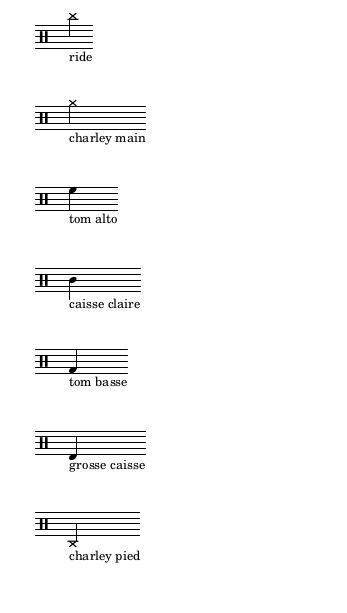
\includegraphics[height=150mm, width=90mm]{images/description_notation_0.png}\\
Il faudra ajouter :
\begin{itemize}
	\item le cross-cut
	\item les ghost-notes
\end{itemize}
\subsection*{Notation des flas}
\textit{À faire :}
\begin{itemize}
	\item Trouver des flas dans les méthodes américaines\\
\end{itemize}
On considère comme un fla deux frappes très proches non-synchrones et qui ne sont pas quantifiées. La première de ces deux notes est une appogiature. En batterie, elle peut-être jouée piano ou avec la même force que la suivante.
L’écriture des flas ressemble à celle des appogiatures même si cette dernière place la note ornementale à un degré (ton ou demi-ton) au-dessus ou au-dessous de la note principale.\footnote{Théorie de la musique, A. Danhauser}
\section*{2. Définition des symboles et des hauteurs}
\subsection*{Proposition de définition d’un standard de départ}
Pour la transcriptions, nous proposons de choisir la base Agostini. La caisse claire centrale sur la portée est aussi centrale sur la batterie est elle est un élément qui conditionne la position des jambes (écart entre les pédales, etc.) ainsi que l’organisation des éléments en hauteur (toms, cymbales, etc.).
On pensera en terme de symétrie la répartition des éléments par rapport au point central que constitue la caisse claire.\\
Cette symétrie s’opère en trois dimensions :
\begin{itemize}
	\item Les hauteurs en terme de fréquences ;
	\item La hauteur physique des éléments :\\
	Du bas vers le haut : pédales, toms et caisse, cymbales
	\item L’ergonomie, qui hiérarchise l’importance des éléments sur la portée (caisse claire au centre, hh-pied et ride sont aux deux extrémités).
\end{itemize}
\section*{3. Direction des hampes et des ligatures}
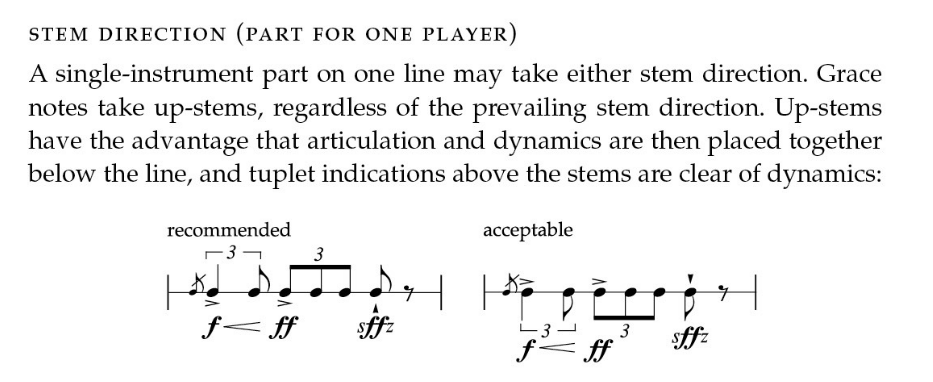
\includegraphics[height=60mm, width=120mm]{images/hampes_0.png} \\\textit{Source : Behind Bars, Elaine Gould}\\\\
Le principe ci-dessus semble être respecté dans les rythmiques binaires de Juskowiac mais pas dans les Méthodes agostini\\

\textbf{Quelques idées :}\\
\begin{itemize}
	\item \textbf{\textit{Les systèmes :}}\\
	$\Rightarrow$ Un système est la combinaison d’un ou plusieurs éléments qui jouent un rythme en boucle (système) et d’un autre élément qui joue un \textit{texte} rythmique variable mais respectant les règles propre au système (texte).\\
	En cas de système, les ligatures forment deux voies :
	\begin{itemize}
		\item Le texte ;
		\item Le système.
	\end{itemize}
	\textit{Mettre des exemples de différents systèmes.}
	\item \textbf{\textit{Les moulins :}}\\
	Lorsqu’il y a plus d’une voie, ils sont prioritaires pour les ligatures.\\
	\textit{Mettre des exemples.}\\
\end{itemize}
—————————————————————————————————————————————————————————————————————————————————————\\\\